\documentclass[crop,tikz]{standalone}

\usepackage{tikz}
\usetikzlibrary{positioning, arrows}
\tikzstyle{line} = [draw, -latex']

\newcommand{\AxisRotator}[1][rotate=0]{%
	\tikz [x=0.25cm,y=0.60cm,line width=.2ex,-stealth,#1] \draw (0,0) arc (150:-150:1 and 0.5);%
}
\newcommand{\AxisRotatorNew}[1][rotate=0]{%
	\tikz [x=0.25cm,y=0.60cm,line width=.2ex,-stealth,#1] \draw (0,0) arc (-150:150:1 and 0.5);%
}


\begin{document}

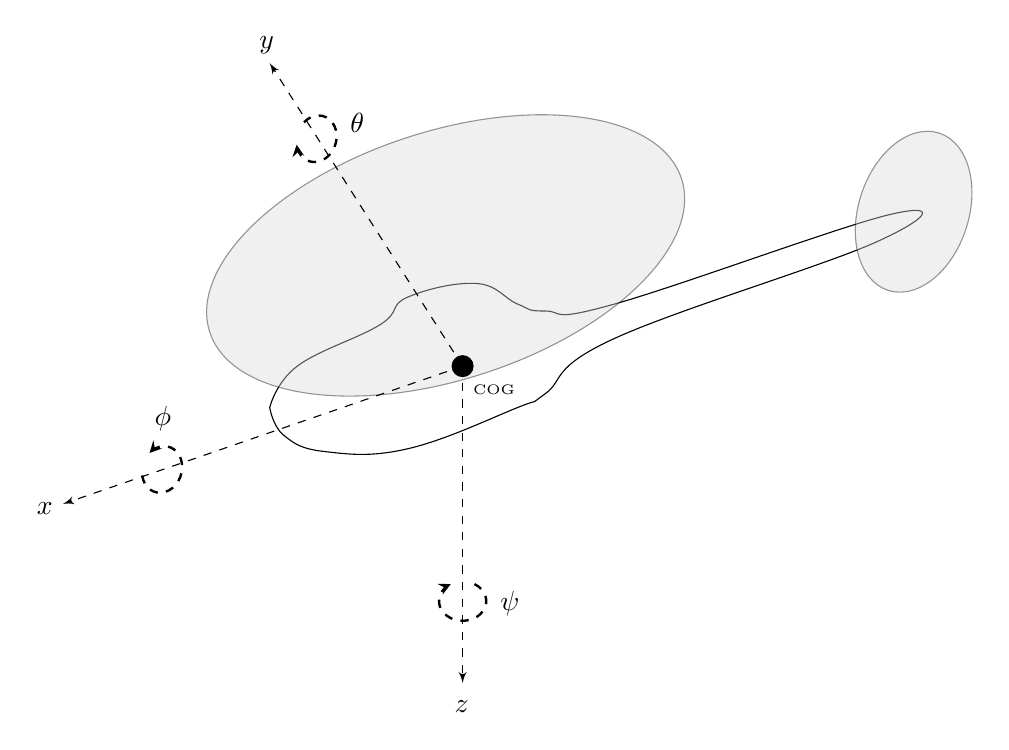
\begin{tikzpicture}[scale=1.75]
\draw  plot[smooth, tension=.7] coordinates {(-5,0) (-4.8,0.3) (-4.2,0.6) (-4,0.8) (-3.5,0.9) (-3.2,0.75) (-3,0.7) (-2.5,0.75) (-0.5,1.4) (-0.6,1.2) (-2.5,0.5) (-3,0.1) (-3.2,0) (-4,-0.3) (-4.6,-0.32) (-4.9,-0.2) (-5,0)};
\draw[rotate=18,fill=gray!30,opacity=0.4] (-3.2,2.2) ellipse (1.8cm and 0.9cm);
\draw[rotate=-18,fill=gray!30,opacity=0.4] (-0.75,1.25) ellipse (0.4cm and 0.6cm);
\draw[fill=black] (-3.6,0.3) circle (0.5ex) node[xshift=0.4cm,yshift=-0.3cm] {\tiny{COG}};
\draw[line,dashed] (-3.6,0.3) -- node[near end,anchor=south,xshift=-1.5cm,yshift=-0.7cm] {$ x $} (-6.5,-0.7) node [near end] {\AxisRotatorNew[rotate=-18]} node [near end,yshift=0.65cm] {$ \phi $};
\draw[line,dashed] (-3.6,0.3) -- node[near end,anchor=east,xshift=0.2cm,yshift=-1.3cm] {$ z $} (-3.6,-2) node [near end] {\AxisRotator[rotate=-90]} node [near end,xshift=0.6cm] {$ \psi $};
\draw[line,dashed] (-3.6,0.3) -- node[near end,anchor=south,xshift=-0.65cm,yshift=0.95cm] {$ y $} (-5,2.5) node [near end] {\AxisRotator[rotate=-18]} node [near end,xshift=0.5cm,yshift=0.2cm] {$ \theta $};
\end{tikzpicture}

\end{document}